\section{An\'{a}lisis descriptivo}
El an\'{a}lisis exploratorio es un proceso que se realiza previamente a la aplicaci\'{o}n de cualquier t\'{e}cnica estad\'{i}stica a un conjunto de datos, la cual tiene por objetivo identificar el comportamiento de los datos a trav\'{e}s del an\'{a}lisis de gr\'{a}ficos y de estad\'{i}stica b\'{a}sica para permitir\'{a} explorar la distribuci\'{o}n de los datos e identificar caracter\'{i}sticas tales como: valores at\'{i}picos o outliers, concentraciones de valores, saltos o discontinuidades, forma de la distribuci\'{o}n, entre otros.   

%Configuración de Clusters de Datos del DANE




\subsection{An\'{a}lisis inicial}
Lo primero que se analizar\'{a} es el comportamiento de los datos en las variables Total Aportantes, G\'{e}nero de los Aportantes y Edad del Aportante; obteniendo los siguientes resultados:
%\vspace{1mm}


\begin{kframe}
\begin{alltt}
\hlstd{dfull} \hlkwb{<-} \hlkwd{data.frame}\hlstd{(}\hlkwc{TotalAportes}\hlstd{=datos}\hlopt{$}\hlstd{AporteMensual,}\hlkwc{Genero}\hlstd{=datos}\hlopt{$}\hlstd{Genero,}\hlkwc{Edad}\hlstd{=datos}\hlopt{$}\hlstd{Edad)}
\hlkwd{stargazer}\hlstd{(dfull,}\hlkwc{type}\hlstd{=}\hlstr{"latex"}\hlstd{,}\hlkwc{title}\hlstd{=}\hlstr{"Total Poblacion Analizada"}\hlstd{)}
\end{alltt}
\end{kframe}
% Table created by stargazer v.5.2 by Marek Hlavac, Harvard University. E-mail: hlavac at fas.harvard.edu
% Date and time: vie, may 27, 2016 - 09:10:29 p.m.
\begin{table}[!htbp] \centering 
  \caption{Total Poblacion Analizada} 
  \label{} 
\begin{tabular}{@{\extracolsep{5pt}}lccccc} 
\\[-1.8ex]\hline 
\hline \\[-1.8ex] 
Statistic & \multicolumn{1}{c}{N} & \multicolumn{1}{c}{Mean} & \multicolumn{1}{c}{St. Dev.} & \multicolumn{1}{c}{Min} & \multicolumn{1}{c}{Max} \\ 
\hline \\[-1.8ex] 
TotalAportes & 9,409 & 67,929.350 & 97,627.870 & 98 & 3,200,000 \\ 
Genero & 30,650 & 1.526 & 0.499 & 1 & 2 \\ 
Edad & 30,650 & 33.513 & 21.200 & 0 & 102 \\ 
\hline \\[-1.8ex] 
\end{tabular} 
\end{table} 


%\vspace{1mm}
{\footnotesize \textbf{Convenciones:} Genero) 1: Mujer, 2: Hombre; Edad) Edad del Aportante Analizado.}

%\vspace{1mm}
El an\'{a}lisis principal de esta investigaci\'{o}n se enfoca en comprobar s\'{i} el monto de los aportes aumenta con relaci\'{o}n a la variable edad del aportante. En la revisi\'{o}n de los datos se evidencia que el valor de la media  est\'{a} m\'{a}s cerca del valor m\'{i}nimo  aportado al sistema de seguridad social colombiano.  Por tal raz\'{o}n se ha hace necesario ampliar el an\'{a}lisis a trav\'{e}s de un gr\'{a}fico para poder visualizar mejor los datos de la variable Edad del Aportante.   

\begin{figure}[H]
	\centering
\begin{knitrout}
\definecolor{shadecolor}{rgb}{0.969, 0.969, 0.969}\color{fgcolor}\begin{kframe}
\begin{alltt}
\hlkwd{ggplot}\hlstd{(datosmonto,}\hlkwd{aes}\hlstd{(Edad),}\hlkwd{label}\hlstd{(}\hlstr{"Edad del Aportante"}\hlstd{))} \hlopt{+} \hlkwd{geom_dotplot}\hlstd{()}
\end{alltt}
\end{kframe}
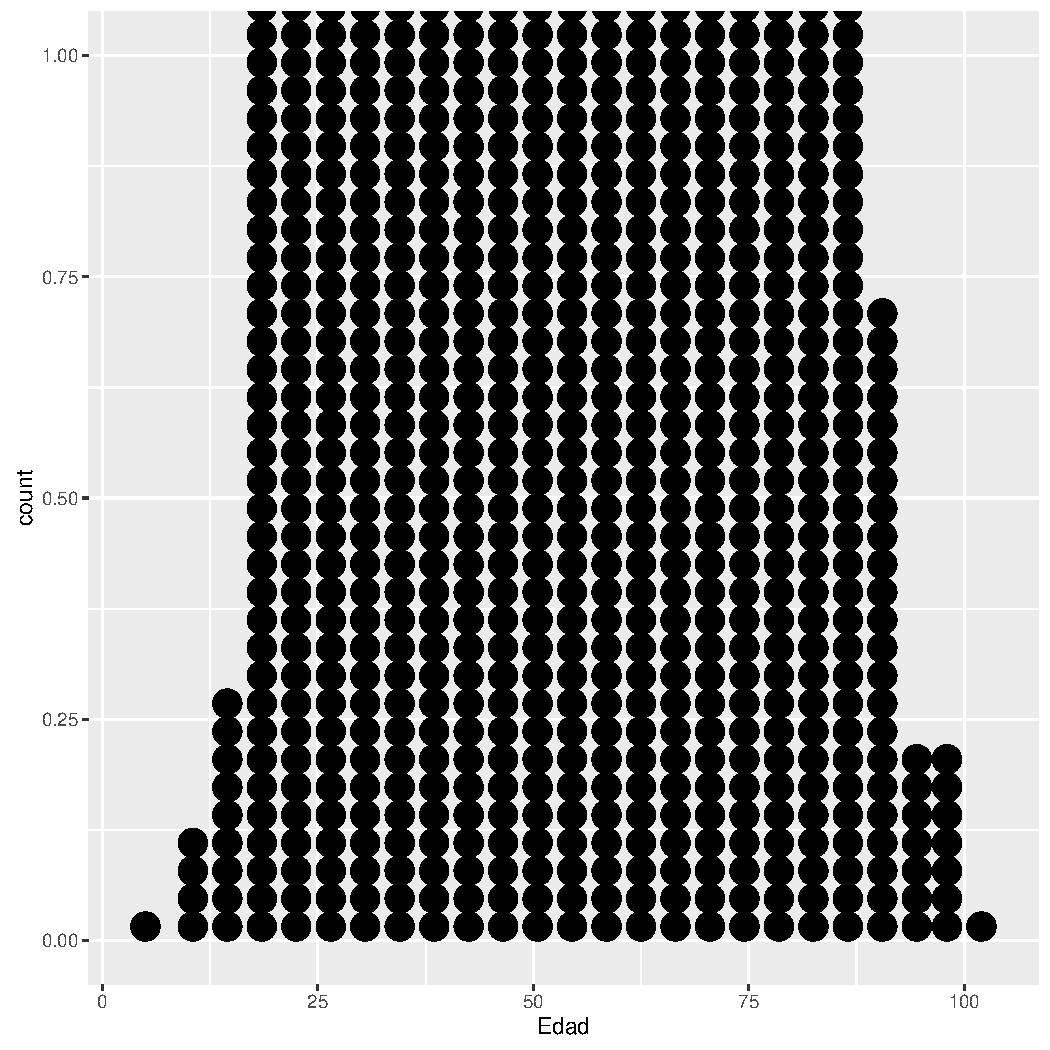
\includegraphics[width=\maxwidth]{figure/EdadAportante-1} 

\end{knitrout}
	\caption{Comportamiento de la variable Edad del Aportante}
\end{figure}

De acuerdo con los datos de la gr\'{a}fica, inicialmente se observan aportes a partir de 22 años, los cuales disminuyen hasta alcanzar 35 años. Posteriormente, el n\'{u}mero de aportante al sistema de seguridad social se mantiene entre el rango de 35 a 45 años.  Luego, la gr\'{a}fica presenta un aumento en el n\'{u}mero de aportantes hasta alcanzar la edad de 60 años. Finalmente, el n\'{u}mero de aportes disminuye hacia los 94 años. En consecuencia, basados en los resultados de los datos, el sistema de seguridad social colombiano est\'{a} financiado por aportes provenientes de ciudadanos que tienen una edad entre 22 hasta 94 años.

Tambi\'{e}n, analizaremos en la siguiente gr\'{a}fica, la distribuci\'{o}n de los datos relacionados con la variable montos de los aportes al sistema de seguridad social, observando lo siguiente:

\begin{figure}[H]
	\centering
\begin{knitrout}
\definecolor{shadecolor}{rgb}{0.969, 0.969, 0.969}\color{fgcolor}\begin{kframe}
\begin{alltt}
\hlkwd{ggplot}\hlstd{(datosmonto,}\hlkwd{aes}\hlstd{(AporteMensual),}\hlkwd{label}\hlstd{(}\hlstr{""}\hlstd{))} \hlopt{+} \hlkwd{geom_dotplot}\hlstd{( )}
\end{alltt}
\end{kframe}
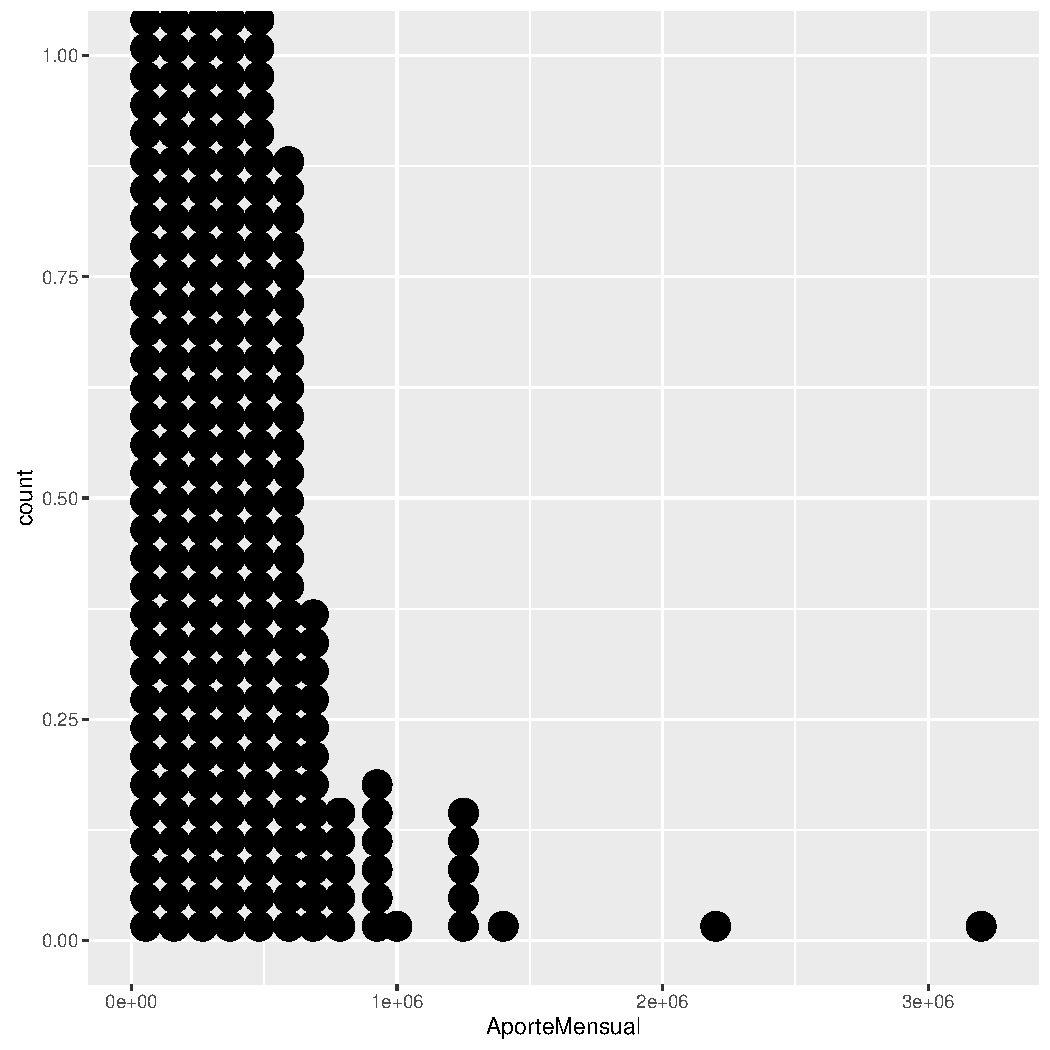
\includegraphics[width=\maxwidth]{figure/MontosAportes-1} 

\end{knitrout}
	\caption{Comportamiento de la variable Monto Aportado al Sistema de Seguridad Social}
\end{figure}

De acuerdo con los datos de la gr\'{a}fica, se observan aportes entre el rango de 98 a 890.000 pesos colombianos.  Los montos de los aportes empiezan con valores menores a la media, es decir 84.000 pesos, posteriormente, se observa el mayor incremento de los aportes en 140.000 pesos y luego comienzan a disminuir hasta los 250.000 pesos colombianos.  Seguidamente, se observan valores alrededor de lo 350.000 y 500.000 pesos colombianos y finalmente, se observa un registro de 890.000 pesos colombianos.  
De acuerdo con los datos observados, los colombianos tiene un aporte bajo al sistema de Seguridad Social y se concentra alrededor de la media es decir 140.000 pesos colombianos.


Con fundamento en los resultados preliminares previos, realizaremos un an\'{a}lisis del conjunto de datos m\'{a}s al detalle, de acuerdo con la informaci\'{o}n disponible.

\vspace{-0mm}
\subsection{Analizando población que aporta al Sistema de Seguridad Social Colombiano cuya edad comprende el rando de 72 hasta 94 años.}

Al comparar la media del total de la poblaci\'{o}n de ciudadanos que aportan al sistema de seguridad social colombiano con la media de la poblaci\'{o}n cuya edad est\'{a} entre 72 a 94 años se observa un incremento de 116.794 pesos colombianos al pasar de 140.206 pesos colombianos a 257.584 pesos colombianos, respectivamente, con lo cual, preliminarmente confirmamos que aumenta el monto de los valores cotizados a este sistema conforme la edad del aportante aumenta. 


%Los datos más representativos se dan a continuación:
\begin{kframe}
\begin{alltt}
\hlstd{d1943} \hlkwb{<-} \hlkwd{data.frame}\hlstd{(}\hlkwc{TotalAportes}\hlstd{=datos1943m}\hlopt{$}\hlstd{AporteMensual,}\hlkwc{Genero}\hlstd{=datos1943m}\hlopt{$}\hlstd{Genero,}\hlkwc{Edad}\hlstd{=datos1943m}\hlopt{$}\hlstd{Edad)}
\hlkwd{stargazer}\hlstd{(d1943,}\hlkwc{type}\hlstd{=}\hlstr{"latex"}\hlstd{,}\hlkwc{title}\hlstd{=}\hlstr{"Total de la población de aportantes al sistema de seguridad social con edad entre 72 y 94 años."}\hlstd{)}
\end{alltt}
\end{kframe}
% Table created by stargazer v.5.2 by Marek Hlavac, Harvard University. E-mail: hlavac at fas.harvard.edu
% Date and time: vie, may 27, 2016 - 09:10:31 p.m.
\begin{table}[!htbp] \centering 
  \caption{Total de la población de aportantes al sistema de seguridad social con edad entre 72 y 94 años.} 
  \label{} 
\begin{tabular}{@{\extracolsep{5pt}}lccccc} 
\\[-1.8ex]\hline 
\hline \\[-1.8ex] 
Statistic & \multicolumn{1}{c}{N} & \multicolumn{1}{c}{Mean} & \multicolumn{1}{c}{St. Dev.} & \multicolumn{1}{c}{Min} & \multicolumn{1}{c}{Max} \\ 
\hline \\[-1.8ex] 
TotalAportes & 638 & 114,674.400 & 124,523.300 & 98 & 1,200,000 \\ 
Genero & 638 & 1.497 & 0.500 & 1 & 2 \\ 
Edad & 638 & 78.423 & 5.696 & 71 & 102 \\ 
\hline \\[-1.8ex] 
\end{tabular} 
\end{table} 


\vspace{1mm}
{\footnotesize \textbf{Convenciones:} Genero) 1: Mujer, 2: Hombre; Edad) Edad del Aportante Analizado.}

De acuerdo con la gr\'{a}fica, se observa un aportante con edad superior a 80 años quien aporta al sistema de seguridad social colombiano. Al comparar el conjunto de datos de los aportes al sistema de seguridad social colombiano con este monto aportado, se observa que este dato tiene una caracter\'{i}stica \'{u}nica por ser quien aport\'{o} el mayor monto al sistema de seguridad social de acuerdo con la informaci\'{o}n analizada. 

%\vspace{0mm}
\begin{figure}[H]
	\centering
\begin{knitrout}
\definecolor{shadecolor}{rgb}{0.969, 0.969, 0.969}\color{fgcolor}\begin{kframe}
\begin{alltt}
\hlkwd{ggplot}\hlstd{(datos1943m,}\hlkwd{aes}\hlstd{(Edad))} \hlopt{+} \hlkwd{geom_histogram}\hlstd{()}
\end{alltt}
\end{kframe}
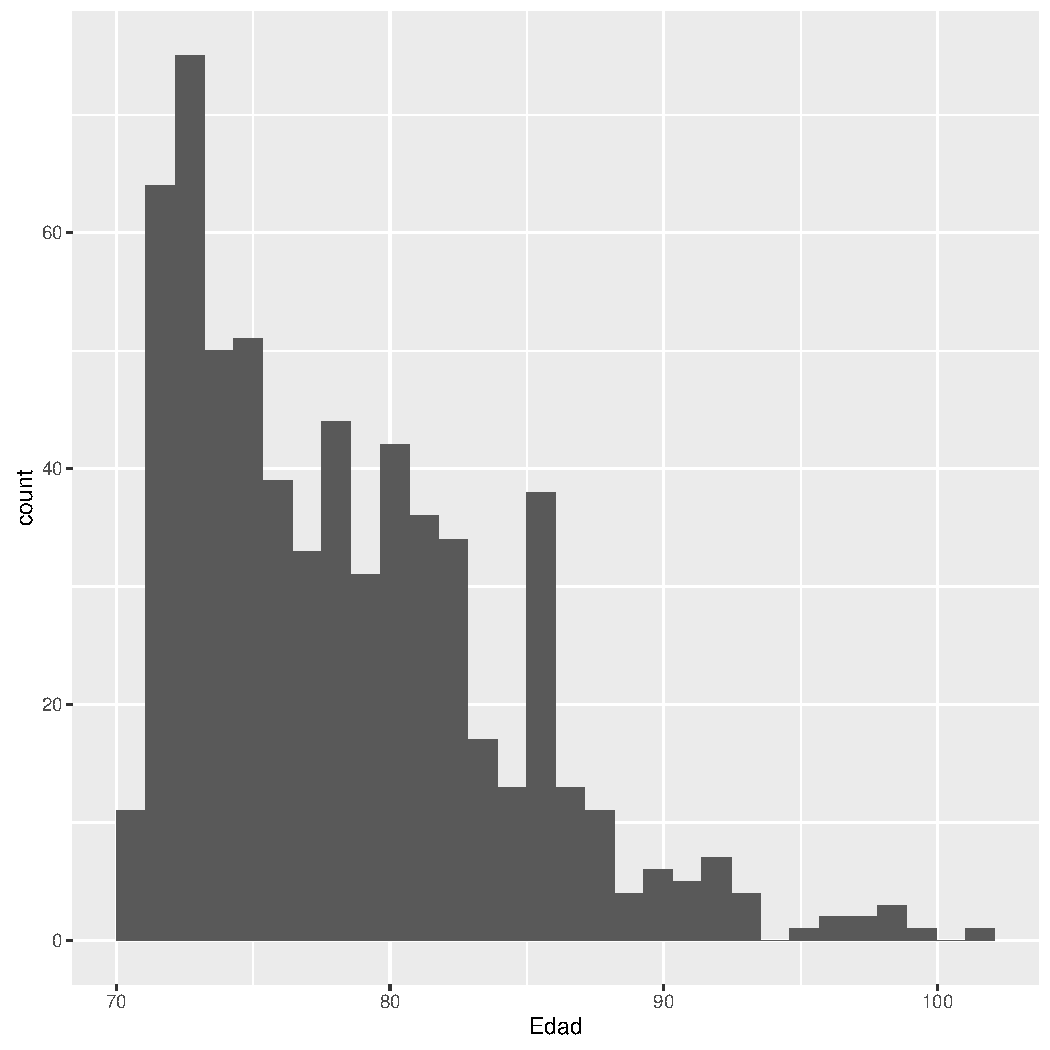
\includegraphics[width=\maxwidth]{figure/Aportantes1943-1} 

\end{knitrout}
	\caption{Población de aportantes del sistema de seguridad social con edad entre 72 y 94 años.}
\end{figure}

Adicionalmente, en la siguiente gr\'{a}fica se observa, que los aportes de los ciudadamos cuya edad est\'{a} entre 72 y 94 años presentan una brecha entre el valor m\'{a}ximo y la media para este rango, existiendo una diferencia de 633.000 pesos colombianos al pasar de 257.000 a 890.000 pesos colombianos, respectivamente.  Tambi\'{e}n, se observa  en la distribuci\'{o}n de los montos aportados, la mayor diferencia entre el menor y el mayor valor aportado, evidenciando la diferencia social de los aportes para esta categor\'{i}a de datos analizados.

Al comparar los datos de la gr\'{a}fica de la variable edad y la variable valor aportado, se observa que la primera tiene una distribuci\'{o}n uniforme, mientras que la segunda evidencia una inclinaci\'{o}n de los datos a la izquierda, concentrado los datos antes de los 250.000 pesos colombianos, y evidenciando que el valor m\'{a}ximo se presenta con poca frecuencia como aporte al sistema social colombiano.   


%\vspace{0mm}
\begin{figure}[H]
	\centering
\begin{knitrout}
\definecolor{shadecolor}{rgb}{0.969, 0.969, 0.969}\color{fgcolor}\begin{kframe}
\begin{alltt}
\hlkwd{ggplot}\hlstd{(datos1943m,}\hlkwd{aes}\hlstd{(AporteMensual))} \hlopt{+} \hlkwd{geom_histogram}\hlstd{()}
\end{alltt}
\end{kframe}
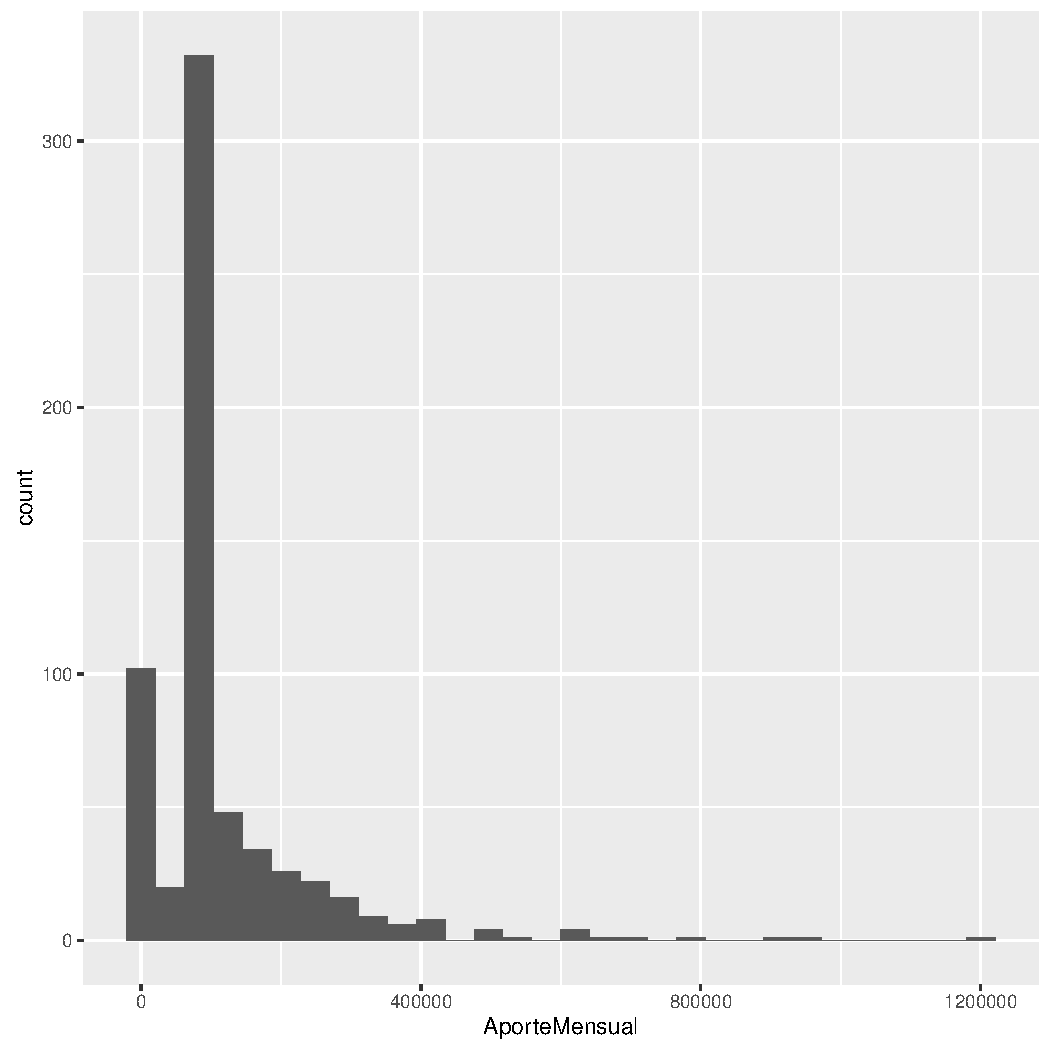
\includegraphics[width=\maxwidth]{figure/MontoAporte1943-1} 

\end{knitrout}
	\caption{Montos de los aportes al sistema de seguridad social de la poblacion con edad entre 72 y 94 años.}
\end{figure}




%\vspace{-10mm}
\subsection{Analizando población  que aporta al Sistema de Seguridad Social Colombiano cuya edad comprende el rango de 50 años y menos de 71 años.}

%Los datos más representativos se dan a continuación:
\begin{kframe}
\begin{alltt}
\hlstd{d1965} \hlkwb{<-} \hlkwd{data.frame}\hlstd{(}\hlkwc{TotalAportes}\hlstd{=datos1965m}\hlopt{$}\hlstd{AporteMensual,}\hlkwc{Genero}\hlstd{=datos1965m}\hlopt{$}\hlstd{Genero,}\hlkwc{Edad}\hlstd{=datos1965m}\hlopt{$}\hlstd{Edad)}
\hlkwd{stargazer}\hlstd{(d1965,}\hlkwc{type}\hlstd{=}\hlstr{"latex"}\hlstd{,}\hlkwc{title}\hlstd{=}\hlstr{"Total de la poblacion de aportantes del sistema de seguridad social con edad entre 50 y 71 años."}\hlstd{)}
\end{alltt}
\end{kframe}
% Table created by stargazer v.5.2 by Marek Hlavac, Harvard University. E-mail: hlavac at fas.harvard.edu
% Date and time: vie, may 27, 2016 - 09:10:31 p.m.
\begin{table}[!htbp] \centering 
  \caption{Total de la poblacion de aportantes del sistema de seguridad social con edad entre 50 y 71 años.} 
  \label{} 
\begin{tabular}{@{\extracolsep{5pt}}lccccc} 
\\[-1.8ex]\hline 
\hline \\[-1.8ex] 
Statistic & \multicolumn{1}{c}{N} & \multicolumn{1}{c}{Mean} & \multicolumn{1}{c}{St. Dev.} & \multicolumn{1}{c}{Min} & \multicolumn{1}{c}{Max} \\ 
\hline \\[-1.8ex] 
TotalAportes & 2,586 & 100,892.100 & 126,888.600 & 98 & 1,400,000 \\ 
Genero & 2,586 & 1.442 & 0.497 & 1 & 2 \\ 
Edad & 2,586 & 58.831 & 6.198 & 49 & 71 \\ 
\hline \\[-1.8ex] 
\end{tabular} 
\end{table} 


\vspace{1mm}
{\footnotesize \textbf{Convenciones:} Genero) 1: Mujer, 2: Hombre; Edad) Edad del Aportante Analizado.}

Al comparar la media del total de la poblaci\'{o}n de ciudadanos que aportan al Sistema de Seguridad Social Colombiano con la media de la poblaci\'{o}n cuya edad est\'{a} entre 50 y 71 años, se observa un incremento de 29.346 pesos colombianos al pasar de 140.206 pesos colombianos a 169.552 pesos colombianos, respectivamente, con lo cual, continua la tendencia, al aumentar el monto de los valores cotizados a este sistema conforme la edad del aportante aumenta. 


Basados en los datos de la siguiente gr\'{a}fica, se observa constancia en el n\'{u}mero de aportantes que existen para el rango de los ciudadanos con edad entre 50 a 59 años, y un incremento en el n\'{u}mero de aportantes en el rango de 60 a 71 años.  Llama la atenci\'{o}n el incremento del n\'{u}mero de aportantes a los 71 años, lo cual corresponden a ciudadanos pensionados por el Sistema de Seguridad Social Colombiano.  

%\vspace{-5mm}
\begin{figure}[H]
	\centering
\begin{knitrout}
\definecolor{shadecolor}{rgb}{0.969, 0.969, 0.969}\color{fgcolor}\begin{kframe}
\begin{alltt}
\hlkwd{ggplot}\hlstd{(datos1965m,}\hlkwd{aes}\hlstd{(Edad))} \hlopt{+} \hlkwd{geom_histogram}\hlstd{()}
\end{alltt}
\end{kframe}
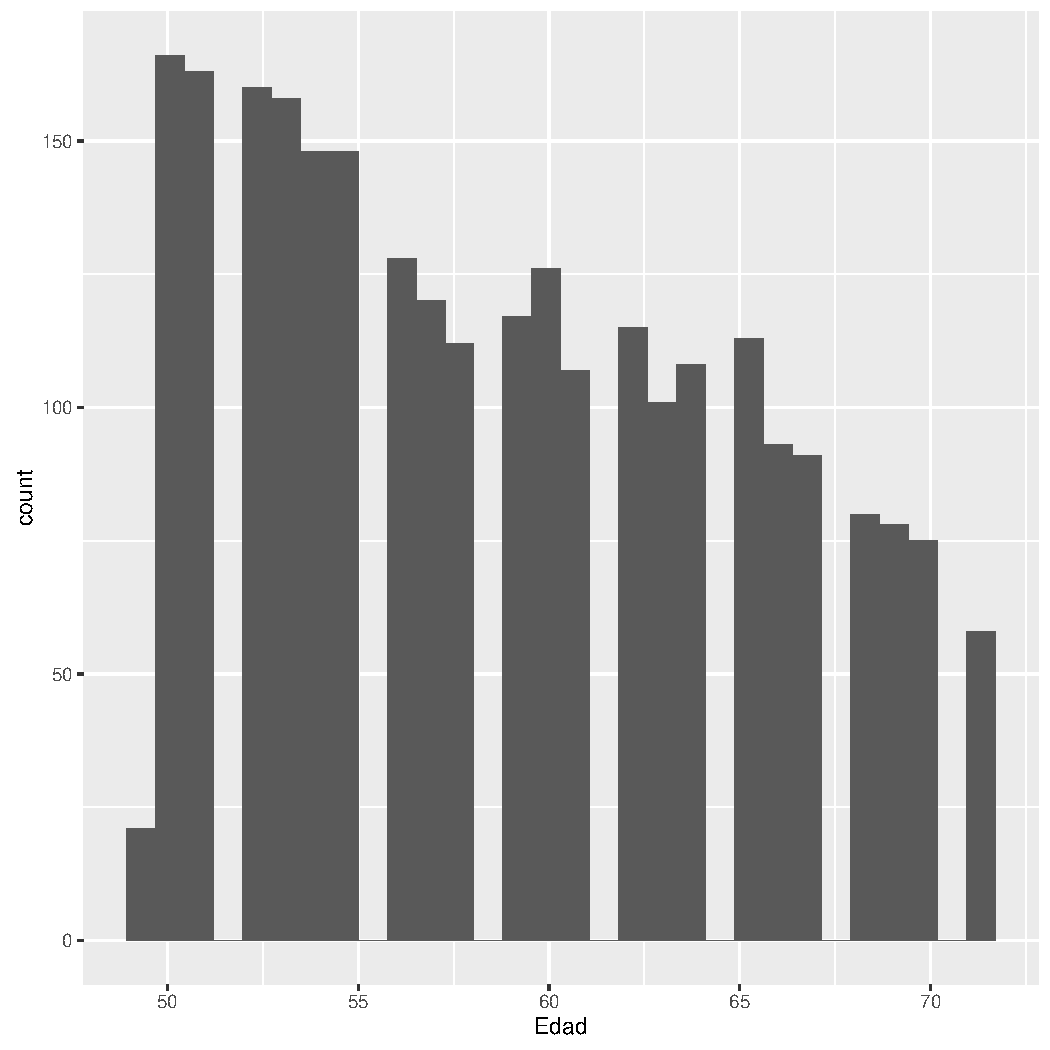
\includegraphics[width=\maxwidth]{figure/Aportantes1965-1} 

\end{knitrout}
	\caption{Población de aportantes del sistema de seguridad social con edad entre 50 y 71 años.}
\end{figure}

Tambi\'{e}n revisaremos la calidad de los aportes realizado al sistema de acuerdo con los datos de este rango, presentados en la siguiente gr\'{a}fica:


%\vspace{-5mm}
\begin{figure}[H]
	\centering
\begin{knitrout}
\definecolor{shadecolor}{rgb}{0.969, 0.969, 0.969}\color{fgcolor}\begin{kframe}
\begin{alltt}
\hlkwd{ggplot}\hlstd{(datos1965m,}\hlkwd{aes}\hlstd{(AporteMensual))} \hlopt{+} \hlkwd{geom_histogram}\hlstd{()}
\end{alltt}
\end{kframe}
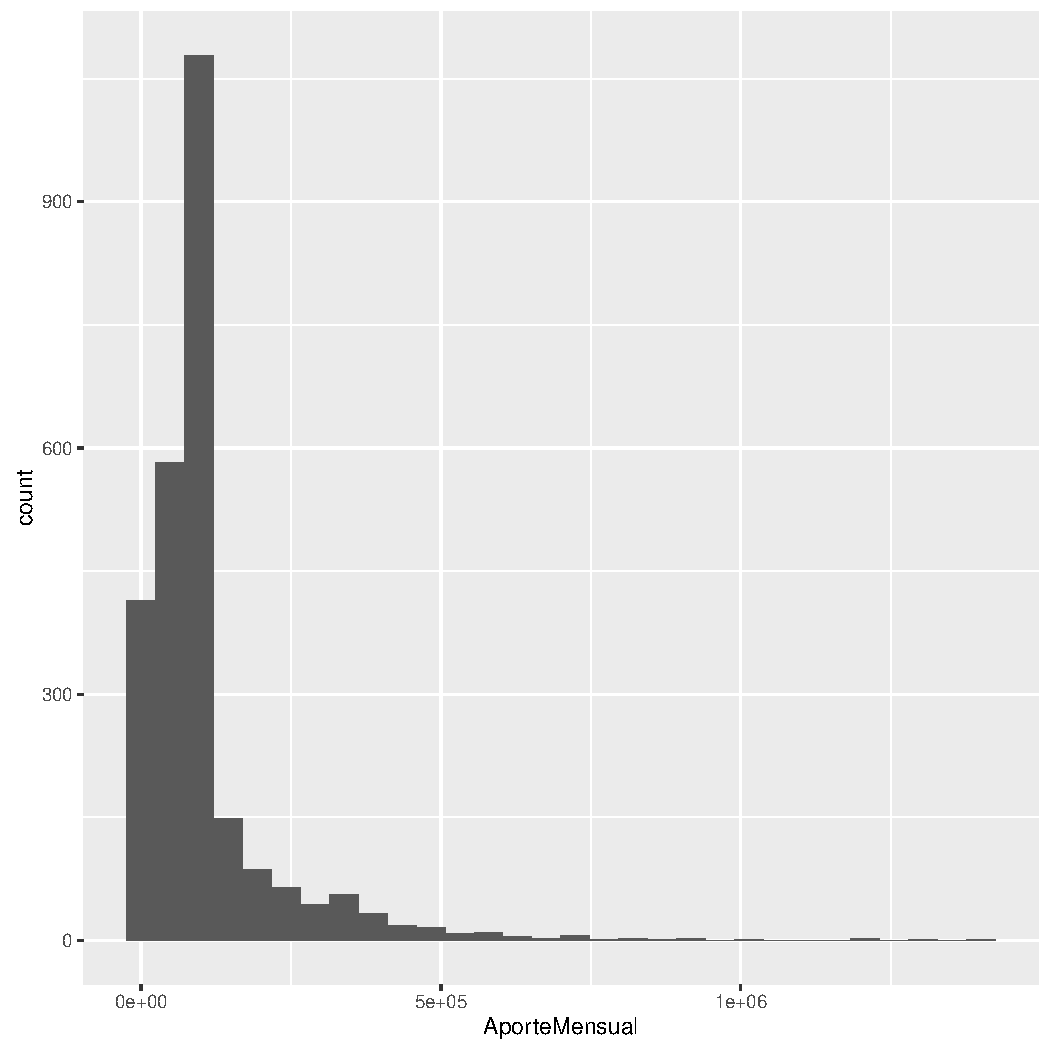
\includegraphics[width=\maxwidth]{figure/Aportantes1965monto-1} 

\end{knitrout}
	\caption{Montos de los aportes al sistema de seguridad social con edad entre 50 y 71 años.}
\end{figure}

Al comparar la media del total de la poblaci\'{o}n de ciudadanos que aportan al Sistema de Seguridad Social Colombiano con la media de la poblaci\'{o}n cuya edad est\'{a} entre 50 a 71 años, se observa un incremento de 29.346 pesos colombianos al pasar de 140.206 pesos colombianos a 169.552 pesos colombianos, respectivamente. 

%\vspace{-10mm}
\subsection{Analizando población de aportantes del sistema de seguridad social con edad entre 27 y 50 años.}
%Los datos más representativos se dan a continuación:
\begin{kframe}
\begin{alltt}
\hlstd{d1988} \hlkwb{<-} \hlkwd{data.frame}\hlstd{(}\hlkwc{TotalAportes}\hlstd{=datos1988m}\hlopt{$}\hlstd{AporteMensual,}\hlkwc{Genero}\hlstd{=datos1988m}\hlopt{$}\hlstd{Genero,}\hlkwc{Edad}\hlstd{=datos1988m}\hlopt{$}\hlstd{Edad)}
\hlkwd{stargazer}\hlstd{(d1988,}\hlkwc{type}\hlstd{=}\hlstr{"latex"}\hlstd{,}\hlkwc{title}\hlstd{=}\hlstr{"Total de la población de aportantes al sistema de seguridad social con edad entre 27 y 50 años."}\hlstd{)}
\end{alltt}
\end{kframe}
% Table created by stargazer v.5.2 by Marek Hlavac, Harvard University. E-mail: hlavac at fas.harvard.edu
% Date and time: vie, may 27, 2016 - 09:10:32 p.m.
\begin{table}[!htbp] \centering 
  \caption{Total de la población de aportantes al sistema de seguridad social con edad entre 27 y 50 años.} 
  \label{} 
\begin{tabular}{@{\extracolsep{5pt}}lccccc} 
\\[-1.8ex]\hline 
\hline \\[-1.8ex] 
Statistic & \multicolumn{1}{c}{N} & \multicolumn{1}{c}{Mean} & \multicolumn{1}{c}{St. Dev.} & \multicolumn{1}{c}{Min} & \multicolumn{1}{c}{Max} \\ 
\hline \\[-1.8ex] 
TotalAportes & 4,632 & 53,685.120 & 79,677.910 & 98 & 3,200,000 \\ 
Genero & 4,632 & 1.444 & 0.497 & 1 & 2 \\ 
Edad & 4,632 & 36.591 & 6.636 & 26 & 49 \\ 
\hline \\[-1.8ex] 
\end{tabular} 
\end{table} 


\vspace{1mm}
{\footnotesize \textbf{Convenciones:} Genero) 1: Mujer, 2: Hombre; Edad) Edad del Aportante Analizado.}

Al comparar la media de los aportes del total de la poblaci\'{o}n de ciudadanos que aportan al Sistema de Seguridad Social Colombiano con la media de la poblaci\'{o}n cuya edad est\'{a} entre 27 a 50 años, se observa un disminuci\'{o}n de 39.408 pesos colombianos al pasar de 140.206 pesos colombianos a 100.798 pesos colombianos, respectivamente, con lo cual, continua la tendencia, al aumentar el monto de los valores cotizados a este sistema conforme la edad del aportante aumenta. 


%\vspace{-5mm}
\begin{figure}[H]
	\centering
\begin{knitrout}
\definecolor{shadecolor}{rgb}{0.969, 0.969, 0.969}\color{fgcolor}\begin{kframe}
\begin{alltt}
\hlkwd{ggplot}\hlstd{(datos1988,}\hlkwd{aes}\hlstd{(Edad))} \hlopt{+} \hlkwd{geom_histogram}\hlstd{()}
\end{alltt}
\end{kframe}
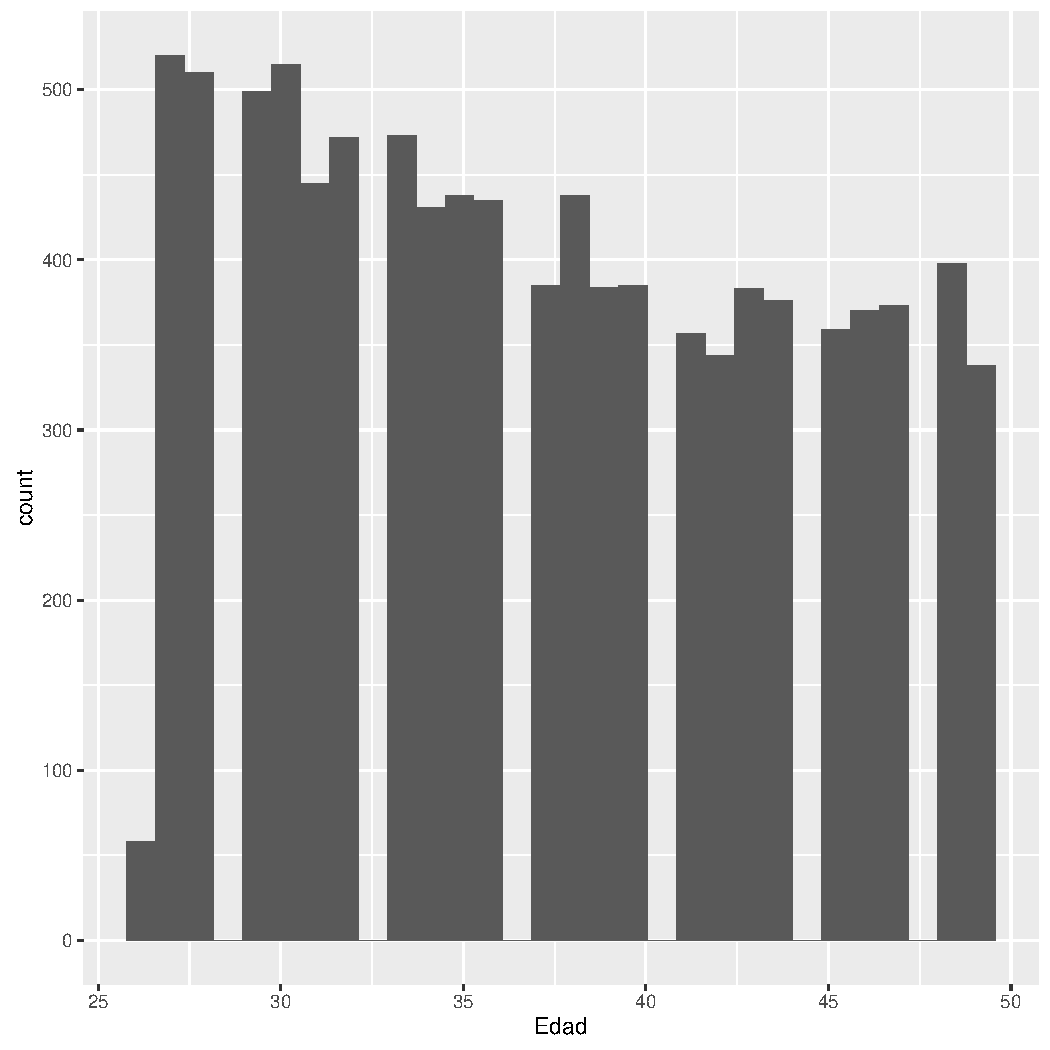
\includegraphics[width=\maxwidth]{figure/Aportantes1988-1} 

\end{knitrout}
	\caption{Población de aportantes del sistema de seguridad social con edad entre 27 y 50 años.}
\end{figure}

Al revisar los montos aportados en este rango, se observa una gr\'{a}fica inclinada a la izquierda, indicando que el valor de los montos est\'{a}n sobre los 100.000 pesos colombianos. Tambi\'{e}n, se observa un \'{u}nico dato de 353,200 para este rango de datos evidenciando una diferencia social entre el m\'{a}ximo valor y la media de los aportes al sistema de seguridad social colombiano en este rango de datos analizado.


%\vspace{-5mm}
\begin{figure}[H]
	\centering
\begin{knitrout}
\definecolor{shadecolor}{rgb}{0.969, 0.969, 0.969}\color{fgcolor}\begin{kframe}
\begin{alltt}
\hlkwd{ggplot}\hlstd{(datos1988m,}\hlkwd{aes}\hlstd{(AporteMensual))} \hlopt{+} \hlkwd{geom_histogram}\hlstd{()}
\end{alltt}
\end{kframe}
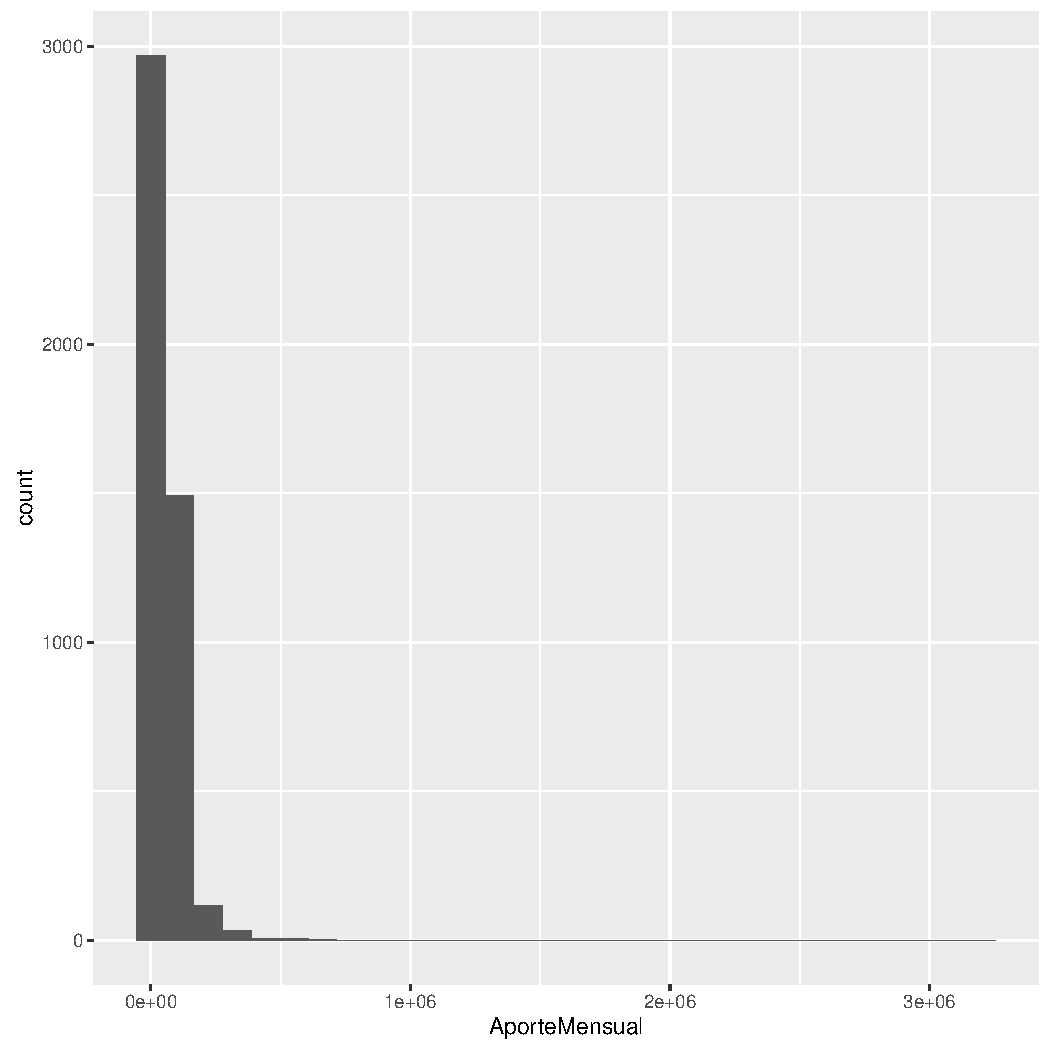
\includegraphics[width=\maxwidth]{figure/Aportantes1988monto-1} 

\end{knitrout}
	\caption{Montos de los aportes al sistema de seguridad social con edad entre 27 y 50 años.}
\end{figure}


%\vspace{-10mm}
\subsection{Analizando población de aportantes del sistema de seguridad social con edad entre 22 y 26 años.}
%Los datos más representativos se dan a continuación:
\begin{kframe}
\begin{alltt}
\hlstd{d1993} \hlkwb{<-} \hlkwd{data.frame}\hlstd{(}\hlkwc{TotalAportes}\hlstd{=datos1993}\hlopt{$}\hlstd{AporteMensual,}\hlkwc{Genero}\hlstd{=datos1993}\hlopt{$}\hlstd{Genero,}\hlkwc{Edad}\hlstd{=datos1993}\hlopt{$}\hlstd{Edad)}
\hlkwd{stargazer}\hlstd{(d1993,}\hlkwc{type}\hlstd{=}\hlstr{"latex"}\hlstd{,}\hlkwc{title}\hlstd{=}\hlstr{"Total de la población de aportantes del sistema de seguridad social con edad entre 22 26 años."}\hlstd{)}
\end{alltt}
\end{kframe}
% Table created by stargazer v.5.2 by Marek Hlavac, Harvard University. E-mail: hlavac at fas.harvard.edu
% Date and time: vie, may 27, 2016 - 09:10:32 p.m.
\begin{table}[!htbp] \centering 
  \caption{Total de la población de aportantes del sistema de seguridad social con edad entre 22 26 años.} 
  \label{} 
\begin{tabular}{@{\extracolsep{5pt}}lccccc} 
\\[-1.8ex]\hline 
\hline \\[-1.8ex] 
Statistic & \multicolumn{1}{c}{N} & \multicolumn{1}{c}{Mean} & \multicolumn{1}{c}{St. Dev.} & \multicolumn{1}{c}{Min} & \multicolumn{1}{c}{Max} \\ 
\hline \\[-1.8ex] 
TotalAportes & 1,149 & 37,639.140 & 38,566.700 & 98 & 644,000 \\ 
Genero & 2,756 & 1.511 & 0.500 & 1 & 2 \\ 
Edad & 2,756 & 23.831 & 1.421 & 21 & 26 \\ 
\hline \\[-1.8ex] 
\end{tabular} 
\end{table} 

\vspace{1mm}
{\footnotesize \textbf{Convenciones:} Genero) 1: Mujer, 2: Hombre; Edad) Edad del Aportante Analizado.}

Basados en los resultados de la tabla anterior, observamos que al comparar la media de los montos aportados al Sistema de Seguridad Social por el total de la poblaci\'{o}n de ciudadanos  con relaci\'{o}n a la media de la poblaci\'{o}n cuya edad est\'{a} entre 22 a 26 años, identificamos una disminuci\'{o}n de 96.616 pesos colombianos al pasar de 140.206 pesos colombianos a 43.587 pesos colombianos, respectivamente, con lo cual, continua la tendencia donde aumenta el monto de los valores cotizados considerando la variable edad del aportante.

Al analizar como es la distribucin\'{o}n de los datos en este rango, analizando la variable edad observamos que existen un mayor n\'{u}mero de  aportantes hacia los 22 años y que el n\'{u}mero de incidencias disminuye hacia los 26 años, como se observa en la siguiente gr\'{a}fica: 

%\vspace{-10mm}
\begin{figure}[H]
	\centering
\begin{knitrout}
\definecolor{shadecolor}{rgb}{0.969, 0.969, 0.969}\color{fgcolor}\begin{kframe}
\begin{alltt}
\hlkwd{ggplot}\hlstd{(datos1993,}\hlkwd{aes}\hlstd{(Edad))} \hlopt{+} \hlkwd{geom_histogram}\hlstd{()}
\end{alltt}
\end{kframe}
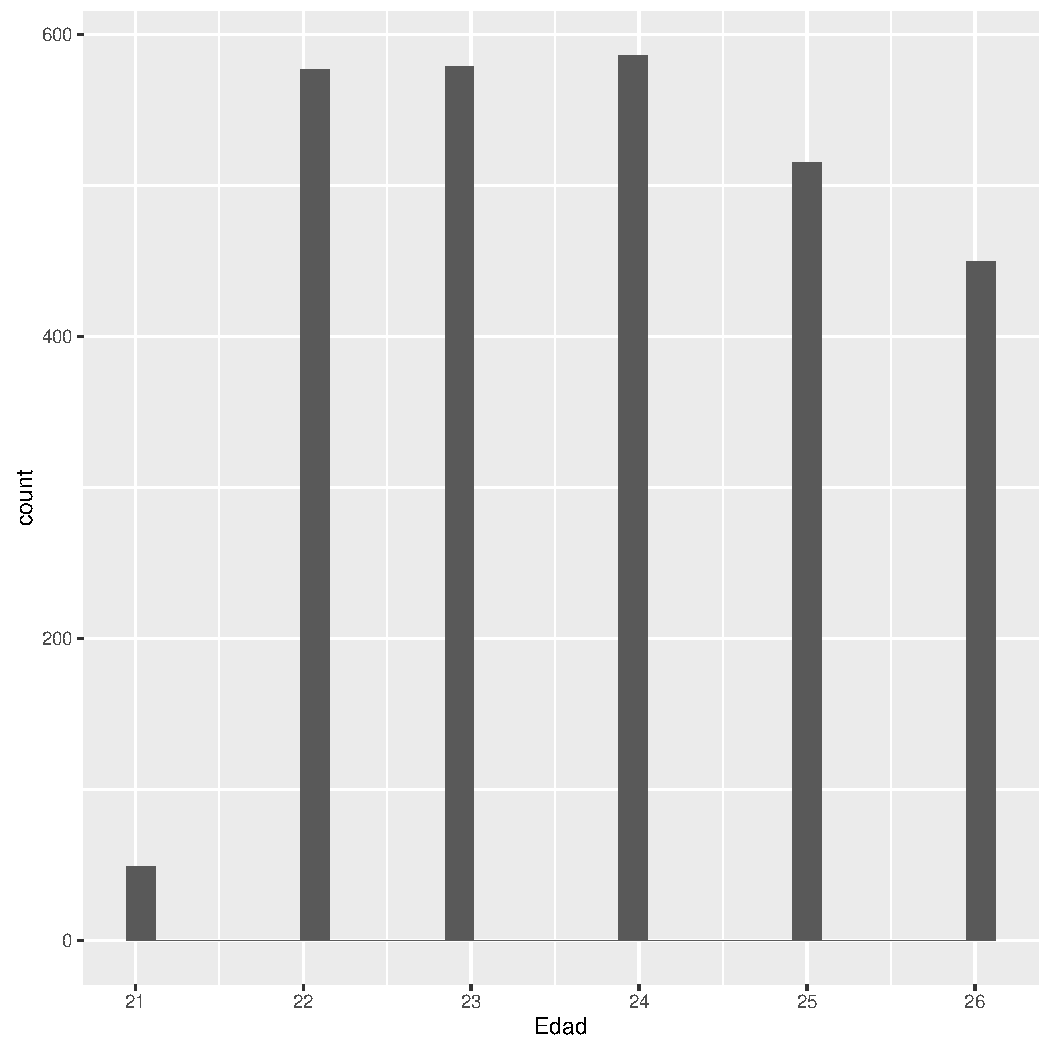
\includegraphics[width=\maxwidth]{figure/Aportantes1993-1} 

\end{knitrout}
	\caption{Población de aportantes del sistema de seguridad social con edad entre 22 y 26 años.}
\end{figure}

Tambi\'{e}n, analizamos el comportamiento de los montos aportados, al sistema observando una inclinaci\'{o}n de los datos hacia  la izquierda, observando una mayor incidencia alrededor de los  25.774 pesos colombianos, como se observa a continuaci\'{o}n.

%\vspace{-10mm}
\begin{figure}[H]
	\centering
\begin{knitrout}
\definecolor{shadecolor}{rgb}{0.969, 0.969, 0.969}\color{fgcolor}\begin{kframe}
\begin{alltt}
\hlkwd{ggplot}\hlstd{(datos1993m,}\hlkwd{aes}\hlstd{(AporteMensual))} \hlopt{+} \hlkwd{geom_histogram}\hlstd{()}
\end{alltt}
\end{kframe}
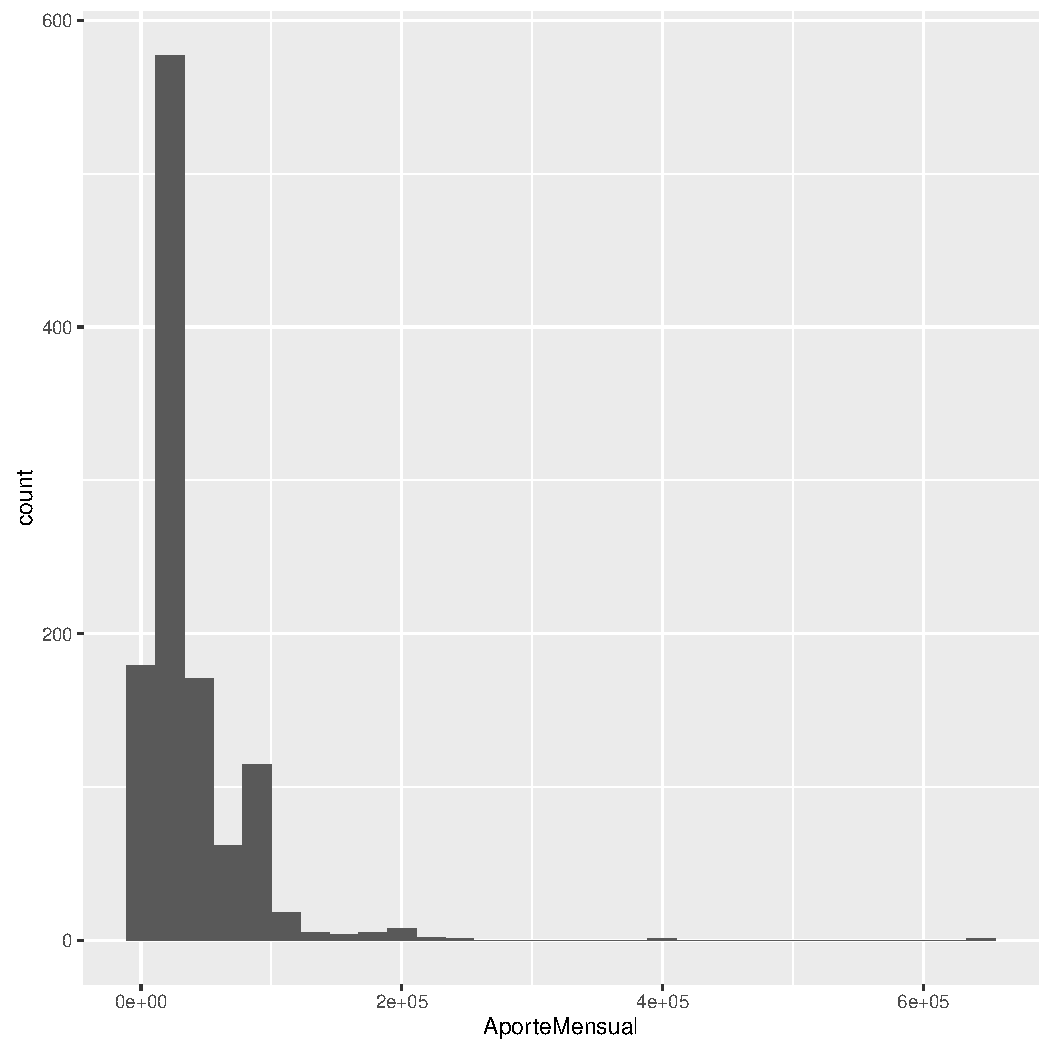
\includegraphics[width=\maxwidth]{figure/Aportantes1993monto-1} 

\end{knitrout}
	\caption{Montos de los aportes del sistema de seguridad social con edad entre 22 y 26 años.}
\end{figure}

Finalmente se presenta los montos aportados al sistema de seguridad social colombiano categorizado por la varible Edad. 

\begin{itemize}
	\item Promedio de montos de los aportes de los ciudadanos entre 22 a 26 años:
[1] 37639.14

	\item Promedio de montos de los aportes de los ciudadanos entre 27 a 50 años:
[1] 53685.12

	\item Promedio de montos de los aportes de los ciudadanos entre 51 a 71 años:
[1] 100892.1

	
	\item Promedio de montos de los aportes de los ciudadanos entre 72 a 94 años:
[1] 114674.4

	
	\item Promedio de montos de los aportes de los ciudadanos al Sistema de Seguridad Social presentado de forma consolidada:
[1] 67929.35

\end{itemize}

\section{An\'{a}lisis Exploratorio}

Revisado los resultados del trabajo realizado observamos que el valor m\'{a}ximo de los aportes realizados por la poblaci\'{o}n colombiana al sistema de seguridad social aumentan con relaci\'{o}n a la variable Edad, al pasar: 

\begin{itemize}
	
	\item  de 82.800 pesos colombianos para el rango de aportantes de 22 a 26  años
	
	
	\item  de 353.200 pesos colombianos para el rango de aportantes de 27 a 50  años
	
	\item  de 492.000 pesos colombianos para el rango de aportantes de 51 a 71  años
	
	\item  de 890.000 pesos colombianos para el rango de aportantes de 72 a 94  años.
	
\end{itemize}

En consecuencia, se puede concluir que existe un n\'{u}mero de ciudadanos a los cuales sus aportes est\'{a}n por encima de la media de los montos de los aportes al sistema y aumentan con relaci\'{o}n a la variable edad. 

\section{An\'{a}lisis Inferencial}

Finalmente, fundamentados en los resultados obtenidos en fases previas, consideramos la pregunta donde se cuestiona s\'{i} los colombianos que m\'{a}s aportan tienen una edad mayor a 30 años, a la cual podemos mencionar:  


\begin{itemize}
	
	\item  La media de los montos aportados al sistema de seguridad social colombiano con datos al 2015, categorizados por rangos, aumentan con relaci\'{o}n a la variable edad.
	
	\item  Los valores m\'{a}ximos de los montos aportados aumentan con relaci\'{o}n a la variable edad.
	
	\item   Al revisar, la gr\'{a}fica que consolida los montos de los aportes de los ciudadanos entre 22 y 26  años se observa una media de 43.587 pesos colombianos y un valor m\'{a}ximo de 82.800 pesos colombianos, respectivamente, con lo cual estos valores son menores a los aportes en otras categor\'{i}as analizados en este papel. 
	
\end{itemize}  

En consecuencia se concluye que los montos aportados al sistema de seguridad social colombiano, por los ciudadanos con edad superior a 30 años es mayor a los montos aportados por la poblaci\'{o}n con una edad menor.

Finalmente, mediante el an\'{a}lisis de la informaci\'{o}n mediante la t\'{e}cnica de miner\'{i}a de datos K-means, el cual permite visualizar el comportamiento de las variables Edad y Monto aportado en Conjunto, as\'{i}: 

\begin{kframe}


{\ttfamily\noindent\bfseries\color{errorcolor}{\#\# Error in eval(expr, envir, enclos): no se pudo encontrar la funci�n "{}geom.dotplot"{}}}\end{kframe}
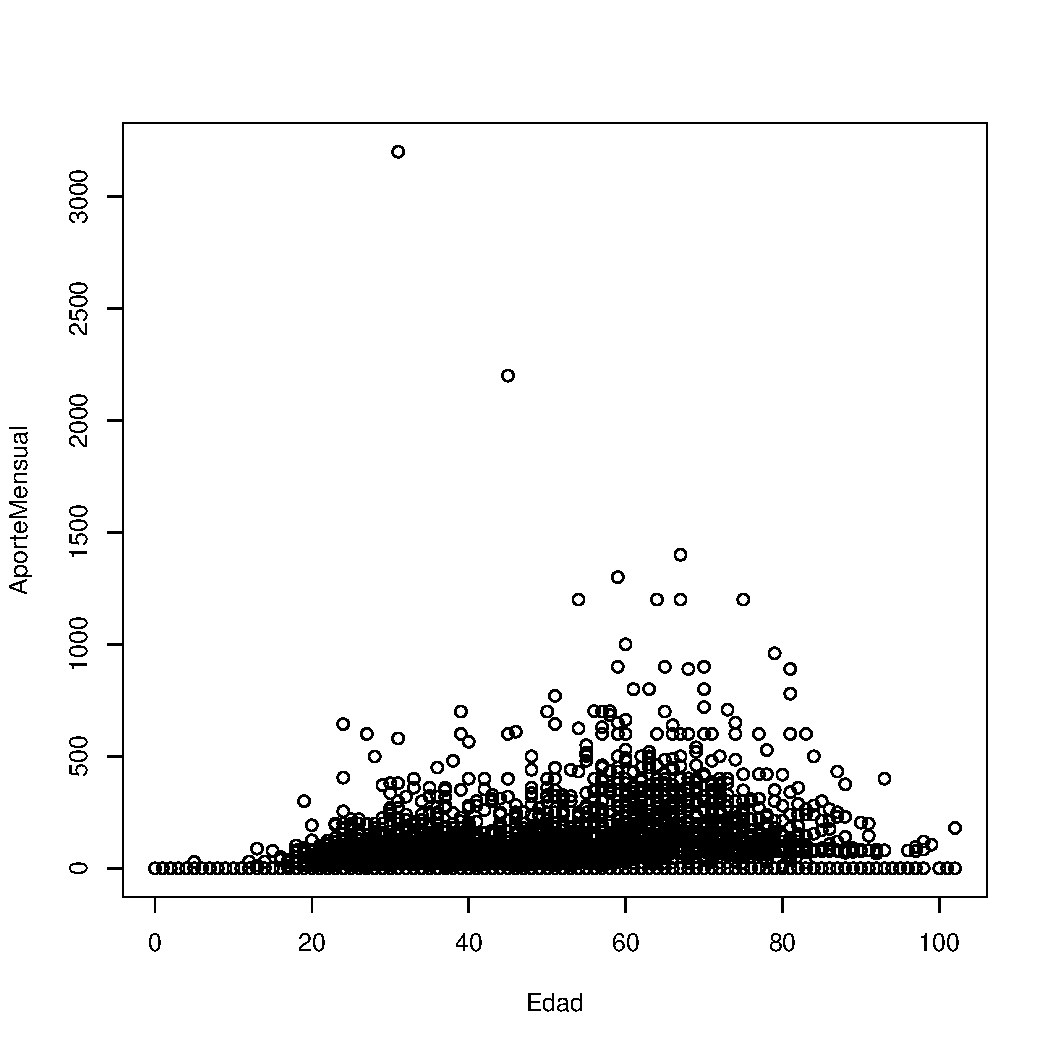
\includegraphics[width=\maxwidth]{figure/medias-1} 



En el eje de las X, se observa la variable edad y en en el eje de la y, se representa la variable de los aportes al sistema, la cual sintetiza el an\'{a}lisis realizado.


\begin{kframe}


{\ttfamily\noindent\bfseries\color{errorcolor}{\#\# Error: no se puede ubicar un vector de tama�o\ \ 3.5 Gb}}

{\ttfamily\noindent\bfseries\color{errorcolor}{\#\# Error in hclust(d): objeto 'd' no encontrado}}

{\ttfamily\noindent\bfseries\color{errorcolor}{\#\# Error in plot(h): objeto 'h' no encontrado}}\end{kframe}


%\vspace{-10mm}
%\subsection{Percentiles del conjunto de datos}
%El percentil de orden \(k\) es el cuantil de orden \(\dfrac {k} {100}\). El recorrido intercuantil refleja la variabilidad de las observaciones comprendidas entre los percentiles 25 y 75 en el conjunto de datos. En esta sesión se obtienen los percentiles del 25\%,  50\% y 75\% de las variables Total Población (TP) y Total Población Hispana (TPH) en los diferentes años de la muestra.

%\vspace{4mm}
%\begin{itemize}
%\item Percentiles del población en el año 1990
%	<<perc1990,results='asis',echo=FALSE, warning=FALSE, message=FALSE>>=
%		grupo1990TP <- c(quantile(datos1990$TP,c(.25)), quantile(datos1990$TP,c(.50)), quantile(datos1990$TP,c(.75)))
%		grupo1990PH <- c(quantile(datos1990$TPH,c(.25)), quantile(datos1990$TPH,c(.50)), quantile(datos1990$TPH,c(.75)))
%		q1990<-data.frame(PercentilesTP=grupo1990TP, PercentilesTPH=grupo1990PH)	 	
%	 	xtable(q1990,"Percentiles de TP y TPH en el año 1990")
%	@

%	<<perc2000,results='asis',echo=FALSE, warning=FALSE, message=FALSE>>=
%		grupo2000TP <- c(quantile(datos2000$TP,c(.25)), quantile(datos2000$TP,c(.50)), quantile(datos2000$TP,c(.75)))
%		grupo2000PH <- c(quantile(datos2000$TPH,c(.25)), quantile(datos2000$TPH,c(.50)), quantile(datos2000$TPH,c(.75)))
%		q2000<-data.frame(PercentilesTP=grupo2000TP, PercentilesTPH=grupo2000PH)	 	
%		xtable(q2000,"Percentiles de TP y TPH en el año 2000")
%	@

%	<<perc2010,results='asis',echo=FALSE, warning=FALSE, message=FALSE>>=
%		grupo2010TP <- c(quantile(datos2010$TP,c(.25)), quantile(datos2010$TP,c(.50)), quantile(datos2010$TP,c(.75)))
%		grupo2010PH <- c(quantile(datos2010$TPH,c(.25)), quantile(datos2010$TPH,c(.50)), quantile(datos2010$TPH,c(.75)))
%		q2010<-data.frame(PercentilesTP=grupo2010TP, PercentilesTPH=grupo2010PH)	 	
%		xtable(q2010,"Percentiles de TP y TPH en el año 2010")
%	@

%	<<perc2011,results='asis',echo=FALSE, warning=FALSE, message=FALSE>>=
%		grupo2011TP <- c(quantile(datos2011$TP,c(.25)), quantile(datos2011$TP,c(.50)), quantile(datos2011$TP,c(.75)))
%		grupo2011PH <- c(quantile(datos2011$TPH,c(.25)), quantile(datos2011$TPH,c(.50)), quantile(datos2011$TPH,c(.75)))
%		q2011<-data.frame(PercentilesTP=grupo2011TP, PercentilesTPH=grupo2011PH)	 	
%		xtable(q2011,"Percentiles de TP y TPH en el año 2011")
%	@
